\documentclass{beamer}

\usepackage{listings}
\usepackage{ulem}
\usepackage{color}

\definecolor{codered}{rgb}{0.69,0.09,0.12}
\definecolor{codegreen}{rgb}{0,0.6,0}
\definecolor{codegray}{rgb}{0.5,0.5,0.5}
\definecolor{codepurple}{rgb}{0.58,0,0.82}
\definecolor{backcolour}{rgb}{0.9,0.9,0.9}
\definecolor{forecolour}{rgb}{0.9,0.9,0.9}

\usepackage{hyperref}
\hypersetup{
    colorlinks = true,
    linkcolor = {codered}
}

\lstdefinestyle{bashstyle}{
    backgroundcolor=\color{backcolour},
    commentstyle=\color{codered},
    keywordstyle=\color{magenta},
    numberstyle=\tiny\color{codegray},
    stringstyle=\color{codepurple},
    basicstyle=\footnotesize,
    breakatwhitespace=false,
    breaklines=true,
    captionpos=b,
    keepspaces=true,
    numbers=left,
    numbersep=5pt,
    showspaces=false,
    showstringspaces=false,
    showtabs=false,
    tabsize=4
}

\lstset{style=bashstyle}

\title{Using Git for Science}

\author{Seb James}
\institute{PSY6422}
\date{2020/05/06}

\begin{document}

\begin{frame}
  \titlepage % makes a title like \maketitle
  Find this at: \url{https://github.com/ABRG-Models/GitTutorial}
\end{frame}

\begin{frame}
  \frametitle{Introduction}
  \begin{itemize}
    \item This session is about a command-line tool called Git.

    \item Git is a tool for managing text, so these slides are naturally text
      heavy!

    \item We'll use it with the help of a website built around Git: github.com

    \item I'll give an overview of Git, including its jargon
      (\alert{clone},\alert{commit},\alert{checkout}...) and why it's
      such a useful tool, then we'll go through some example tasks together.
  \end{itemize}
\end{frame}

\begin{frame}
  \frametitle{What is Git?}
  Git is a \alert{Revision Control} or \alert{Version Control} tool.

  Revision control has two main features:

  \begin{enumerate}
    \pause \item Revision control allows you to have different versions of a
      single file \emph{without having to explicitly make copies}
      \pause \item Most revision control tools allow several people to work
      on the same files %\pause with (non-magic) algorithms that (usually) correctly merge changes
  \end{enumerate}
\end{frame}

\begin{frame}
  \frametitle{File versions}
  I bet you have folders that look like this:
  \pause \begin{itemize}
  \item Project1/myProgram.r
    \pause \item Project1/myProgram\_old.r
  \item Project1/myProgram\_1.r
  \item Project1/myProgram\_thisOneWorked.r
  \item Project1/myProgram\_whoKnowsWhatThisOneIs.r
  \end{itemize}
  \pause With revision control, you only have
  \begin{itemize}
  \item Project1/myProgram.r
  \end{itemize}
\end{frame}

\begin{frame}
  \frametitle{File versions}
  \begin{columns}[T]
    \begin{column}{.5\textwidth}
      \begin{itemize}
      \item Ellipses are folders (aka directories)
      \item Boxes are files
      \end{itemize}
    \end{column}
    \begin{column}{.5\textwidth}
      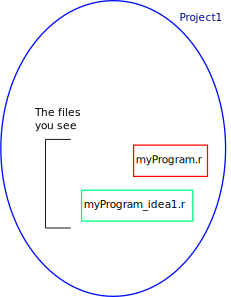
\includegraphics[width=\textwidth]{before_git.png}
    \end{column}
  \end{columns}
\end{frame}

\begin{frame}
  \frametitle{A file with a view}
  \begin{columns}[T]
    \begin{column}{.5\textwidth}
      \begin{itemize}
      \item Git presents a \emph{view} of the file
      \item Versions of the file not being viewed are stored away (in
        \alert{.git})
      \end{itemize}
    \end{column}
    \begin{column}{.5\textwidth}
      \includegraphics[width=\textwidth]{with_git1.png}
    \end{column}
  \end{columns}
\end{frame}

\begin{frame}
  \frametitle{A file with a view}
  \begin{columns}[T]
    \begin{column}{.5\textwidth}
      \begin{itemize}
      \item Git presents a \emph{view} of the file
      \item Versions of the file not being viewed are stored away (in
        \alert{.git})
      \end{itemize}
    \end{column}
    \begin{column}{.5\textwidth}
      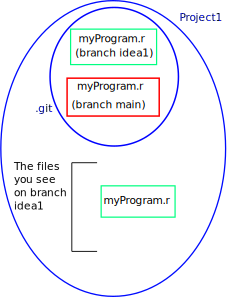
\includegraphics[width=\textwidth]{with_git2.png}
    \end{column}
  \end{columns}
\end{frame}


% SHA1. 40 chars: 525e2104bc8f30057a1e5d264b51be6f113f7181
% Each one is 4 bits, so it's a 160 bit hash with >10^48 values

% The main branch slide
\begin{frame}
  \frametitle{Branches instead of file versions}
  \begin{columns}[T]
    \begin{column}{.5\textwidth}
      When you use git, you use \alert{branches} to work with
      different file versions. There's one central branch, which
      is usually called \textbf{main}.
      \begin{block}{Clone}
        \begin{itemize}
        \item When you \alert{clone} a repository from github, you'll get all
         \textbf{myProgram.r} as it exists on the \textbf{main} branch

        \item Also you get \emph{all the information needed} to see \textbf{myProgram.r}
          on any of the other branches (each has a name)
        \end{itemize}
      \end{block}
    \end{column}
    \begin{column}{.5\textwidth}
      \includegraphics[width=\textwidth]{tree.png}
    \end{column}
  \end{columns}
\end{frame}

% The main branch with increments/commits
\begin{frame}
  \frametitle{A sequence of changes on main}
  \begin{columns}[T]
    \begin{column}{.5\textwidth}
      \begin{block}{Commits}
        \begin{itemize}
          \item There can be different versions of myProgram.r available on
            \textbf{main}; but it's a \emph{sequence of changes}.

          \item Each change is a \alert{commit to main}.

          \item Each commit has a \emph{universally unique identifier}.

          \item When you first clone, you'll see the files at the \alert{HEAD}
            of \textbf{main}
        \end{itemize}
      \end{block}
    \end{column}
    \begin{column}{.5\textwidth}
      \includegraphics[width=\textwidth]{tree_mastercommits_head.png}
    \end{column}
  \end{columns}
\end{frame}

% About what a commit includes
\begin{frame}
  \frametitle{What's in a commit?}
  \begin{columns}[T]
    \begin{column}{.4\textwidth}
      \begin{block}{Commits contain changes}
        \begin{itemize}
        \item One commit can include the changes to one file
        \item One commit can also include changes to multiple files
        \item Each commit has a \alert{commit message}
        \end{itemize}
      \end{block}
    \end{column}
    \begin{column}{.6\textwidth}
      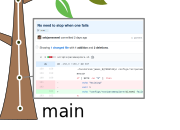
\includegraphics[width=\textwidth]{tree_mastercommits_commitdetail.png}
    \end{column}
  \end{columns}
\end{frame}

% Branch one
\begin{frame}
  \frametitle{Checkout a branch}
  \begin{columns}[T]
    \begin{column}{.5\textwidth}
      \begin{block}{Checkout}
        When you \alert{checkout} a branch, it updates your file to the
        content it has on that particular branch
        \begin{itemize}
          \item Checkout \textbf{idea1}; get myProgram.r with the code for
            your first idea.
          \item Checkout \textbf{paper2\_sub1}; get myProgram.r as it was
            when you submitted your second paper based on the project.
        \end{itemize}
      \end{block}
    \end{column}
    \begin{column}{.5\textwidth}
      
\includegraphics[width=\textwidth]{tree_branchcommits.png}
    \end{column}
  \end{columns}
\end{frame}

% Merge
\begin{frame}
  \frametitle{Merge a branch}
  \begin{columns}[T]
    \begin{column}{.5\textwidth}
      Here's where the tree analogy begins to break down a little.
      \begin{itemize}
      \item Here, a bug was fixed on \textbf{bug\_issue4}. While that was
        happening, someone committed an important commit onto main
      \item To bring the bug fix into main, the \textbf{bug\_issue4}
        branch is \alert{merged} into \textbf{main} which creates its own
        commit
      \end{itemize}
    \end{column}
    \begin{column}{.5\textwidth}
      
\includegraphics[width=\textwidth]{tree_merge.png}
    \end{column}
  \end{columns}
\end{frame}

% Rebase
\begin{frame}
  \frametitle{Rebase a branch}
  \begin{columns}[T]
    \begin{column}{.5\textwidth}
      \begin{block}{Rebase means get out the saw}
        The developer of the bug in \textbf{bug\_issue4} wants to test the bug
        fix works alongside the urgent commit.
      \end{block}
    \end{column}
    \begin{column}{.5\textwidth}
      
\includegraphics[width=\textwidth]{tree_rebase.png}
    \end{column}
  \end{columns}
\end{frame}
% Rebase 2
\begin{frame}
  \frametitle{Rebase a branch}
  \begin{columns}[T]
    \begin{column}{.5\textwidth}
      \begin{block}{\alert{Rebase} means get out the saw}
        The developer of the bug in \textbf{bug\_issue4} wants to test the bug
        fix works alongside the urgent commit.
        \begin{itemize}
          \item Git has a way to `saw off' the branch  \textbf{bug\_issue4}
            and `glue it back onto main'
        \end{itemize}
      \end{block}
    \end{column}
    \begin{column}{.5\textwidth}
      \includegraphics[width=\textwidth]{tree_rebase2.png}
    \end{column}
  \end{columns}
\end{frame}
% Rebase 3
\begin{frame}
  \frametitle{Rebase a branch}
  \begin{columns}[T]
    \begin{column}{.5\textwidth}
      \begin{block}{Rebase means get out the saw}
        The developer of the bug in \textbf{bug\_issue4} wants to test the bug
        fix works alongside the urgent commit.
        \begin{itemize}
          \item Git has a way to `saw off' the branch  \textbf{bug\_issue4}
            and `glue it back onto main'
          \item Now the bug can be tested, alongside the recent change in
            \textbf{main}, before it is then merged into \textbf{main}.
            \item Prefer merge over rebase
        \end{itemize}
      \end{block}
    \end{column}
    \begin{column}{.5\textwidth}
      \includegraphics[width=\textwidth]{tree_rebase3.png}
    \end{column}
  \end{columns}
\end{frame}

\begin{frame}
  \frametitle{Working with other people}

    This is `main feature 2'. Now, rewind a little, forget the trees, and
    think about working with a set of plain files on your computer.


  \begin{itemize}
    \item Suppose you have some code which is used by yourself and 5 of your
      colleagues - some sort of library.

    \pause \item You find an error and fix it. Now you have to email the fix to \emph{5} people.

    \pause \item Just after you emailed them, you find an error in your fix, and you
    have to send another email...

    \pause \item Now imagine that one of your colleagues found a
    separate fix in the same file and emails that around. Which fix is
    more important? Who is going to merge the two fixes together?
  \end{itemize}

  This is where a central copy of the repository becomes important.
\end{frame}

% Pull
\begin{frame}
  \frametitle{Fetch and pull}
  \begin{columns}[T]
    \begin{column}{.5\textwidth}
      Now imagine there is a shared tree living at github.com.
      \begin{block}{Fetch}
        When you \alert{fetch} new changes to the \alert{repo}, information
        about new branches and commits that were added are copied into your
        local copy of the repo.
        \begin{itemize}
        \item Any of the existing branches could have extended
        \item New branches could have appeared
        \item You can \alert{pull} a branch and that will always do a
          \alert{fetch} first
        \end{itemize}
      \end{block}
    \end{column}
    \begin{column}{.5\textwidth}
      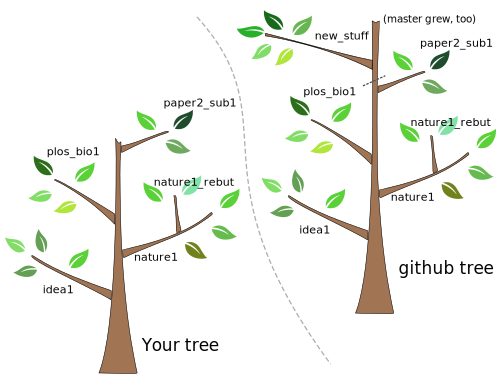
\includegraphics[width=\textwidth]{tree_newbranches.png}
    \end{column}
  \end{columns}
\end{frame}

% Push
\begin{frame}
  \frametitle{Push your commits}
  You worked on a new feature, using a new branch. You changed some existing
  files and added some new ones. You're ready to copy that back to github.com.
  \begin{block}{Push}
    The process of copying new commits and branches as achieved with git \alert{push}.
    \begin{itemize}
    \item You make sure you have \alert{committed} your changes to your branch
    \item You \alert{push} your branch to the online repository (i.e. github)
    \item If there are changes on your branch on the online repository that you don't
      have yet, then you'll have to pull first, \alert{merge} changes and
      \emph{then} push.
    \end{itemize}
  \end{block}
\end{frame}

\begin{frame}
  \frametitle{Other revision control systems}
  Git is not the only game in town. Others include:

  \begin{itemize}
  \item RCS (Revision Control System)
  \item SCCS (Source Code Control System)
  \item CVS (Concurrent Versions System)
  \item Subversion
  \item Tons of proprietary systems
  \item Bazaar
  \item BitKeeper
  \item Mercurial
  \end{itemize}

  \pause Git is not the first revision control system, and its
  developers could draw on a lot of collective knowledge when
  designing it.
\end{frame}

\begin{frame}
  \frametitle{Why did someone develop Git?}
  \begin{itemize}
    \pause \item Most revision control tools have been pretty good at
    feature 1 (file versioning)
    \pause \item ...but not great at managing multiple contributions
    \pause \item That caused Linus Torvalds to commit heresy and use the
    \alert{proprietary} BitKeeper from 2002 to manage the Linux code base.
    \pause \item In 2005 Linus fell out with BitMover Inc., and Git was
    created to replace it (and so all was well again in the world of free
    software OS development - git is fully free).
    \pause \item The name \emph{git} doesn't really mean anything.
  \end{itemize}
\end{frame}

\begin{frame}
  \frametitle{What's different about Git?}
  \begin{itemize}
  \item Git is a \emph{distributed} revision control system
    \pause \item It doesn't have the classical client-server architecture...
    \pause \item When you \alert{clone} a repository from a source, you have
    \emph{everything} (all the file history and meta-data) in those
    files to become a source for someone else.
    \pause \item That means you can work on your code, making incremental
    \alert{commits} even when you don't have internet access.
  \item And every copy of the \alert{repo} is a backup!
  \pause \item It also means you can `\alert{fork}' a repository
    \pause \item Typically you will work with a common
    \alert{remote} repository (github) as your \alert{upstream} source.
  \end{itemize}
\end{frame}

\begin{frame}
  \frametitle{Git is \emph{not} github.com}
  \begin{itemize}
  \item Github is a commercial website which makes it easy to use Git
  \item bitbucket.org is an alternative
  \pause \item Generally, public hosting is free, \sout{private hosting
  incurs a fee}
  \pause \item It's pretty easy to host a git repository yourself, but
  the nice web interface has made github.com very
  popular for source code hosting
  \pause \item It's now a big business; it was acquired by Microsoft in 2018
  \end{itemize}
\end{frame}

\begin{frame}
  \frametitle{Why is Git good for us?}
  We don't have hundreds of people working on the same files, and
  often our work is carried out individually, but...
  \begin{itemize}
    \pause \item We write code, so that's very natural to hold in
    revision control
    \pause \item We store experimental data which is valuable and needs to be
    protected
    \pause \item We write papers about the data and the code
    \pause \item We have a frequent need to \alert{tag} our work (e.g. to
    match up with a paper or document)
    \pause \item ``It used to work, but now I've broken it and I can't
    get it back to working again'': Revision control makes it easy to
    revert to a version of your code which you know will work
    \pause \item You can include your paper (and your data) alongside your model code
    in a single, public repository
    \item Use of Github is a very effective way to share your
    published models with your peers
  \end{itemize}
\end{frame}

\begin{frame}
  \begin{columns}[T]
    \begin{column}{.5\textwidth}
      \frametitle{The rest of the session}
      \begin{itemize}
      \item Create repository on github, clone, add something
      \item git add, git move, git remove, git branch -D etc
      \item git checkout -b newbranch
      \item Github READMEs and markdown
      \item Github issues
      \item doxygen and codedocs.xyz
      \item Demonstration of branches for papers (BarrelEmerge)
      \end{itemize}
    \end{column}
    \begin{column}{.5\textwidth}

      For a good hands-on tutorial, head over to:

      \url{http://sebjameswml.github.io/git-novice/}

      or try the more up to date version of that `Software Carpentry' resource
      at:

      \url{http://swcarpentry.github.io/git-novice/}

    \end{column}
  \end{columns}
\end{frame}

\end{document}
